% !TEX root = ../main.tex
\section{Experiments}
\label{sec:experiments}

\subsection{Setup}
\label{sec:exp:setup}

\paragraph{Benchmark.}
We evaluate on the airline and retail domains of \taubench~\citep{barres2025tau2}, using all \StdPlanned{} tasks that specify gold actions.
As in prior work on speculative tool dispatch~\citep{bai2026spork,anon2026eta}, the user's request is given in a single message, and the agent then works on its own until it replies to the user or has used eight turns.
The tools run against the benchmark's database, and the main comparison uses a tool latency floor of \ToolLowFloor\,s.

\paragraph{Model and serving.}
The agent is Qwen3-32B~\citep{qwen2025qwen3} with reasoning enabled and greedy decoding, served by vLLM~\citep{kwon2023vllm} on four RTX~3090 GPUs.
Prompt-lookup speculative decoding~\citep{saxena2023pld} is enabled for all configurations, so every baseline already benefits from token-level speculation.
We report two serving modes.
For \emph{deterministic serving}, we enable batch-invariant kernels~\citep{he2025nondeterminism} and compare the generated tokens across configurations on the same server instance.
Under \emph{standard serving}, the server uses its default kernels.
Decoding is about three times faster (\SpdStdMsSolo{} instead of \SpdDetMsSolo\,ms per token), but the output of a request can change with the batch, so configurations follow different trajectories.

\paragraph{Configurations.}
\emph{No speculation} is the serial loop.
\emph{Speculative tool dispatch} adds self-speculative probes, early execution of the predicted call, and the reuse of probe tokens as drafts~\citep{bai2026spork}; dispatched calls run on an environment copy as in \cref{sec:method:sandbox}.
\method adds the successor on top of speculative tool dispatch.
The three configurations share the server, the prompts, the decoding settings, and the history policy (\cref{app:impl}).

\paragraph{Protocol and metrics.}
Each task is run once per configuration under deterministic serving and twice under standard serving.
The order of the configurations rotates across tasks, and the server's prefix cache is cleared before every run.
Both serving modes cover all \DetPlanned{} tasks. The ablation uses the \AblIdentPlanned{} tasks in the prespecified validation and test splits.
For the latency sweep we take the \AblTasks{} tasks that completed under every ablation configuration and repeat them at floors of \ToolMidFloor{} and \ToolHighFloor\,s on the same deterministic server.
We measure the end-to-end time of a task, including all waiting and cleanup.
A run fails when a turn reaches the limit of 8{,}192 generated tokens.
Latency is compared on the tasks that all configurations complete, and failures are reported separately.
The \emph{saving} of one configuration over another is the relative reduction of the total time.
Intervals are 95\% bootstrap intervals over tasks.
We score action matching by dividing the number of matched gold actions by the number of gold actions across the paired runs.

\subsection{End-to-End Latency}
\label{sec:exp:latency}

\begin{table*}[t]
\centering
\small
\begin{tabular}{llrrrll}
\toprule
 & & & & & \multicolumn{2}{c}{Saving (\%) over} \\
\cmidrule(lr){6-7}
Serving & Configuration & Mean (s) & P50 (s) & P95 (s) & no speculation & tool dispatch \\
\midrule
Deterministic & No speculation & \DetMeanNone & \DetMedNone & \DetTailNone & -- & -- \\
(\DetTasks{} tasks) & Speculative tool dispatch & \DetMeanDisp & \DetMedDisp & \DetTailDisp & \DetSaveDispNone{} [\DetSaveDispNoneLo, \DetSaveDispNoneHi] & -- \\
 & \method & \DetMeanOurs & \DetMedOurs & \DetTailOurs & \DetSaveOursNone{} [\DetSaveOursNoneLo, \DetSaveOursNoneHi] & \DetSaveOursDisp{} [\DetSaveOursDispLo, \DetSaveOursDispHi] \\
\midrule
Standard & No speculation & \StdMeanNone & \StdMedNone & \StdTailNone & -- & -- \\
(\StdTasks{} tasks, & Speculative tool dispatch & \StdMeanDisp & \StdMedDisp & \StdTailDisp & \StdSaveDispNone{} [\StdSaveDispNoneLo, \StdSaveDispNoneHi] & -- \\
\StdGroups{} pairs) & \method & \StdMeanOurs & \StdMedOurs & \StdTailOurs & \StdSaveOursNone{} [\StdSaveOursNoneLo, \StdSaveOursNoneHi] & \StdSaveOursDisp{} [\StdSaveOursDispLo, \StdSaveOursDispHi] \\
\bottomrule
\end{tabular}
\caption{End-to-end time per task of Qwen3-32B on \taubench. Savings are relative reductions of the total time, with 95\% bootstrap intervals over tasks.}
\label{tab:main}
\end{table*}

Under deterministic serving, \method reduces the mean task time from \DetMeanDisp\,s to \DetMeanOurs\,s.
This is a saving of \DetSaveOursDisp\% over speculative tool dispatch (\DetSpeedOursDisp$\times$) and of \DetSaveOursNone\% over no speculation (\DetSpeedOursNone$\times$).
The median falls by \DetMedSaveOursDisp\% and the 95th percentile by \DetTailSaveOursDisp\%, and \method is faster on \DetFasterOursDisp{} of the \DetTasks{} tasks (\cref{fig:results}a).
Speculative tool dispatch alone saves \DetSaveDispNone\%, because the tool latency that it hides is small next to the reasoning time (\cref{sec:motivation:slack}).

Under standard serving the order is the same and the savings are smaller: \StdSaveOursDisp\% over speculative tool dispatch (\StdSpeedOursDisp$\times$) and \StdSaveOursNone\% over no speculation (\StdSpeedOursNone$\times$).
The configurations follow different trajectories here, so part of each difference is chance in how much the agent generates.
Dividing the time by the number of tokens in the final trajectory removes this part: per token, \method saves \StdTokSaveOursDisp\% [\StdTokSaveOursDispLo, \StdTokSaveOursDispHi] over speculative tool dispatch and \StdTokSaveOursNone\% [\StdTokSaveOursNoneLo, \StdTokSaveOursNoneHi] over no speculation.
\Cref{sec:exp:analysis} relates the gap between the two serving modes to the cost of decoding two requests at once and to the shorter turns under standard serving.

\begin{figure*}[t]
\centering
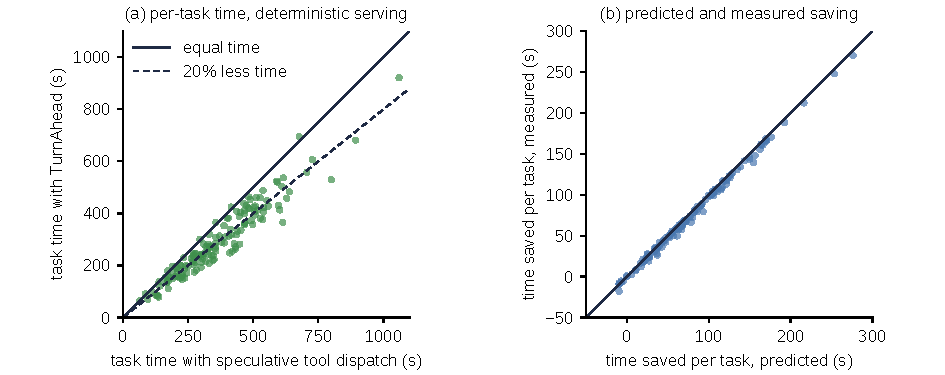
\includegraphics[width=0.92\textwidth]{figures/fig3_results.pdf}
\caption{Deterministic serving, one point per task. (a) Task time with \method against task time with speculative tool dispatch. (b) Time that \method saves over speculative tool dispatch: prediction of the cost model of \cref{sec:exp:analysis}, computed from the dispatch-only run, against the measurement.}
\label{fig:results}
\end{figure*}


\subsection{Trajectory Fidelity and Task Quality}
\label{sec:exp:fidelity}

\paragraph{Deterministic serving.}
On the \DetIdentClean{} tasks that complete, the generated tokens of all \DetIdentTurns{} turns are identical across the configurations, and so are the tool calls, the observations, and the environment after every turn.
The other \DetIdentFailed{} tasks reach the token limit in the same turn, after the same tokens, in every configuration.
The ablation variants also match. Comparing each task and configuration with its own \ToolLowFloor\,s run, all \ToolMidIdentical{} trajectories at \ToolMidFloor\,s and all \ToolHighIdentical{} at \ToolHighFloor\,s reproduce the generated tokens, calls, observations, and database states.
All three configurations match \DetMatchOurs\% of the gold actions on completed tasks.
The sandbox was exercised in these runs: successors changed the database before their check in \MotStateTotal{} windows, \MotStateDiscarded{} of which ended in a discard, and no trace of a discarded change appears in a committed environment.

\paragraph{Standard serving.}
Under standard serving the complete token sequence matches in \StdSameOursDisp{} of \StdSamePairsOursDisp{} successful TurnAhead--dispatch pairs.
The share of gold actions performed is \StdMatchNone\% without speculation, \StdMatchDisp\% with speculative tool dispatch, and \StdMatchOurs\% with \method; \method and speculative tool dispatch differ by \StdMatchDiffOursDisp{} points [\StdMatchDiffOursDispLo, \StdMatchDiffOursDispHi].
The token limit is reached in \StdFailNone, \StdFailDisp, and \StdFailOurs{} of \StdRunsOurs{} runs, respectively; here the two differ by \StdFailDiffOursDisp{} points [\StdFailDiffOursDispLo, \StdFailDiffOursDispHi].

\subsection{Ablation Study}
\label{sec:exp:ablation}

\begin{table}[t]
\centering
\small
\setlength{\tabcolsep}{4pt}
\begin{tabular}{lrl}
\toprule
Variant & Mean (s) & Saving (\%) \\
\midrule
Speculative tool dispatch & \AblMeanDisp & -- \\
\method & \AblMeanOurs & \AblSaveOurs{} [\AblSaveOursLo, \AblSaveOursHi] \\
\quad deferred tools & \AblMeanDefer & \AblSaveDefer{} [\AblSaveDeferLo, \AblSaveDeferHi] \\
\quad no successor probes & \AblMeanNoProbe & \AblSaveNoProbe{} [\AblSaveNoProbeLo, \AblSaveNoProbeHi] \\
\quad start after check & \AblMeanLate & \AblSaveLate{} [\AblSaveLateLo, \AblSaveLateHi] \\
\bottomrule
\end{tabular}
\caption{Variants of \method under deterministic serving (\AblTasks{} tasks). Savings are relative to speculative tool dispatch.}
\label{tab:ablation}
\end{table}

\Cref{tab:ablation} isolates the contributions of early launch, sandboxed tools, and successor probes at the \ToolLowFloor\,s floor.

\paragraph{Start after the check.}
This variant builds the same successor input but runs the check first and starts the successor only if it passes, so parent and successor never overlap.
Its saving vanishes (\AblSaveLate\%).
The gain of \method thus comes entirely from running the next turn inside the parent's slack, and the bookkeeping of a window costs almost nothing.

\paragraph{Deferred tool execution.}
This is the mode of \cref{sec:method:sandbox} that holds the successor's tool calls until the commit decision.
It is \AblSlowerDefer\% slower than the full method [\AblSlowerDeferLo, \AblSlowerDeferHi].

\paragraph{No probes in the successor.}
Without speculative tool dispatch inside the successor, the successor's own tool call is no longer overlapped with its reasoning.
This variant is \AblSlowerNoProbe\% slower than the full method [\AblSlowerNoProbeLo, \AblSlowerNoProbeHi].

Longer tool calls increase the value of probing inside the successor. Removing these probes slows \method by \ToolMidNoProbe\% at \ToolMidFloor\,s and \ToolHighNoProbe\% at \ToolHighFloor\,s. Deferring successor tools until commit has a smaller cost at the same floors (\ToolMidDefer\% and \ToolHighDefer\%). Deferral delays a tool only when the successor reaches it before the parent commits.

\subsection{When Does \method Help?}
\label{sec:exp:analysis}

\paragraph{Windows.}
Under deterministic serving, a successor is started in \WinDetStarted{} of \WinDetWindows{} windows and committed in \WinDetCommitted{} of them (\WinDetCommitPct\%).
Of the \WinDetDiscarded{} discarded successors, \WinDetRejReply{} belong to parents that replied to the user instead of calling a tool and \WinDetRejCall{} to parents that emitted a different call.
The remaining \WinDetRejInput{} belong to parents whose call matched but whose output added something to the history, so that only the input check rejected them.
Under standard serving the commit rate is \WinStdCommitPct\% (\WinStdCommitted{} of \WinStdStarted{} successors).

\paragraph{The cost of a second request.}
While parent and successor overlap, they share the server.
We measure the cost of sharing separately, by decoding the same prompts alone and two at a time (\cref{app:impl}).
Each of two concurrent requests is slowed by a factor of $s=\ConDetTwo$ under deterministic serving and $s=\ConStdTwo$ under standard serving.
According to \cref{sec:method:overview}, a committed window then saves $(2-s)\,\Delta T_t$, and a discarded one costs $(s-1)$ times its overlap.
We apply this model to the runs of speculative tool dispatch, which contain no successors, and predict from them what \method should save (\cref{app:results}).
The prediction is \CostDetPred\% under deterministic serving, where we measure \CostDetMeasured\%, and \CostStdPred\% under standard serving, where we measure \CostStdMeasured\%.
Per task, the predicted and the measured savings under deterministic serving correlate with $r=\CostDetCorr$ (\cref{fig:results}b).

The model also accounts for the gap between the two serving modes.
Without contention ($s=1$) it gives \CostDetIdeal\% and \CostStdIdeal\%.
This part of the gap lies in the workload: turns are shorter under standard serving, so the fixed tool latency takes a larger part of them (the observation is ready after \MotStdReadyPosPct\% of a turn instead of \MotReadyPosPct\%), and fewer turns dispatch a correct call (\MotStdAnchorPct\% instead of \MotAnchorPct\%).
Contention then removes \CostDetContention{} points under deterministic serving and \CostStdContention{} under standard serving.
The second request adds a similar time per token in both modes (\ConDetExtraMs\,ms and \ConStdExtraMs\,ms), which is a larger fraction when a single request decodes faster.
Committed successors account for \WinDetOverlapCommitPct\% of observed overlap time under deterministic serving and \WinStdOverlapCommitPct\% under standard serving. Both exceed the respective break-even shares of \CostDetBreakeven\% and \CostStdBreakeven\%.

\paragraph{Overhead.}
\method generates more tokens than it commits.
Counting probes and discarded successors, speculative tool dispatch generates \OvhDetGenDisp{} tokens per committed token and \method generates \OvhDetGenOurs.
Discarded successors alone amount to \OvhDetLostPctOurs\% of the committed tokens (\OvhStdLostPctOurs\% under standard serving).
On a dedicated server this work uses capacity that the serial loop leaves idle, and its effect on latency is already part of the measured times.

\paragraph{Can discarded work be reused?}
A discarded successor could serve as a token-level draft for the turn that replaces it.
The replaced turns hold \ReuseDetReplacedPct\% of the committed tokens.
Runs of at least eight tokens that a replaced turn shares with its discarded successor cover \ReuseDetSharedPct\% of its tokens, which is \ReuseDetSharedAllPct\% of all committed tokens (\ReuseStdSharedAllPct\% under standard serving).
A successor is usually discarded because the parent decided otherwise, and it then reasons about an observation that the real turn never sees.

\paragraph{Tool latency.}
Longer tool calls shift the gain toward early dispatch (\cref{fig:tool-latency}). Raising the floor from \ToolLowFloor{} to \ToolHighFloor\,s increases the saving of dispatch over serial execution from \ToolLowDispatch\% to \ToolHighDispatch\%.
The observation also arrives later, leaving less parent reasoning in which to run a successor. The additional saving over dispatch falls from \ToolLowIncrement\% to \ToolMidIncrement\% and then \ToolHighIncrement\%.
Together, dispatch and early successor execution save \ToolLowTotal\%, \ToolMidTotal\%, and \ToolHighTotal\% over serial execution at the three floors.

\begin{figure}[t]
\centering
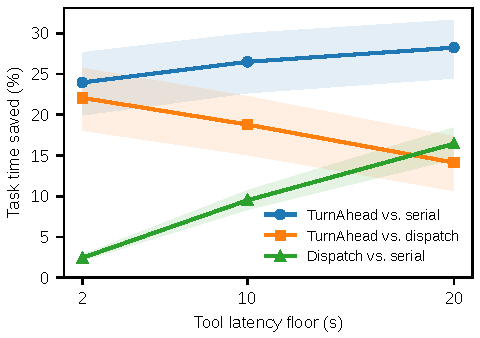
\includegraphics[width=\columnwidth]{figures/fig4_tool_latency.pdf}
\caption{Task time saved as tool latency increases on the same \AblTasks{} tasks. Shading gives task-bootstrap 95\% intervals.}
\label{fig:tool-latency}
\end{figure}
